% tikzlibrarysstknots.code.tex
\ProvidesFile{tikzlibrarysstknots.code.tex}[2025/09/01 SST knot helpers]

\RequirePackage{tikz}
\usetikzlibrary{knots,hobby,calc,intersections,decorations.pathreplacing,shapes.geometric,spath3}

% ------- Shared styles (from your preamble) -------
\tikzset{
    knot diagram/every strand/.append style={ultra thick, black},
    every path/.style={black,line width=2pt},
    every node/.style={transform shape,knot crossing,inner sep=1.5pt},
    every knot/.style={line cap=round,line join=round,very thick},
    strand/.style={line cap=round,line join=round,line width=3pt,draw=black},
    over/.style={preaction={draw=white,line width=6.5pt}},
    sst/ring A/.style={draw=black, line width=3pt},
    sst/ring B/.style={draw=black,  line width=3pt},
    sst/ring C/.style={draw=black, line width=3pt},
}

% ------- Guides toggle -------
\newif\ifsstguides
\sstguidesfalse

% ------- Helper: label & skeleton for points P1..Pn -------
\newcommand{\SSTGuidesPoints}[2]{% #1=basename (e.g. P), #2=last index
    \ifsstguides
    \foreach \i in {1,...,#2}{
        \fill[blue] (#1\i) circle (1.2pt);
        \node[blue,font=\scriptsize,above] at (#1\i) {\i};
    }
    \draw[gray!40, dashed] \foreach \i [remember=\i as \lasti (initially 1)] in {2,...,#2,1} { (#1\lasti)--(#1\i) };
    \fi
}

% ====================================================================
% LATEX SWIRL STRING THEORY
% KNOT LIBRARY
% ====================================================================

% --------------------------------------------------------------------
% 6_1: Down Quarck Stevedore
% Usage: \SSTdown
% --------------------------------------------------------------------
\newcommand{\SSTdown}[1][2,4,6,8]{% optional arg = flip list
    \begin{tikzpicture}[use Hobby shortcut]
        \coordinate (P1)  at ( 0,  1.5);
        \coordinate (P2)  at (-2,  2);
        \coordinate (P3)  at (-1.5, 0);
        \coordinate (P4)  at ( 1, -1.5);
        \coordinate (P5)  at (-1.5,-2);
        \coordinate (P6)  at (-2.5,-0.5);
        \coordinate (P7)  at (-1.5, 1);
        \coordinate (P8)  at ( 0,  3);
        \coordinate (P9)  at ( 1.5, 1);
        \coordinate (P10) at ( 2.5,-0.5);
        \coordinate (P11) at ( 1.5,-2);
        \coordinate (P12) at (-1, -1.5);
        \coordinate (P13) at ( 1.5, 0);
        \coordinate (P14) at ( 2,  2);
        \coordinate (P15) at ( 0,  1.5); % = P1

        \begin{knot}[
            consider self intersections,
            clip width=5pt, clip radius=3pt,
            ignore endpoint intersections=false,
            flip crossing/.list={#1}
        % draft mode=crossings % uncomment to see numbers
        ]
        \strand
        ([closed] P1)..(P2)..(P3)..(P4)..(P5)..(P6)..(P7)..(P8)%
        ..(P9)..(P10)..(P11)..(P12)..(P13)..(P14)..(P15);
        \end{knot}
        \SSTGuidesPoints{P}{15}
    \end{tikzpicture}%
}


% --------------------------------------------------------------------
% 5_2: Up Quark
% Usage: \SSTup
% --------------------------------------------------------------------
\newcommand{\SSTup}[1][2,4,6,8]{% optional arg = flip list
    \begin{tikzpicture}[use Hobby shortcut]
        \coordinate (P1) at ( 2.0,  2.0);
        \coordinate (P2) at ( 1.8,  0.0);
        \coordinate (P3) at (-2.3, -1.0);
        \coordinate (P4) at ( 0.5,  1.0);
        \coordinate (P5) at (-2.0,  2.0);
        \coordinate (P6) at (-1.8,  0.0);
        \coordinate (P7) at ( 2.3, -1.0);
        \coordinate (P8) at (-0.5,  1.0);
        \coordinate (P9) at ( 2.0,  2.0); % = P1

        \begin{knot}[
            consider self intersections,
            clip width=5pt, clip radius=3pt,
            ignore endpoint intersections=false,
            flip crossing/.list={#1}
        % draft mode=crossings
        ]
        \strand
        ([closed] P1)..(P2)..(P3)..(P4)..(P5)..(P6)..(P7)..(P8)..(P9);
        \end{knot}
        \SSTGuidesPoints{P}{9}
    \end{tikzpicture}%
}

% --------------------------------------------------------------------
% Usage: \SSTSeptfoil
% --------------------------------------------------------------------
\newcommand{\SSTSeptfoil}{%
    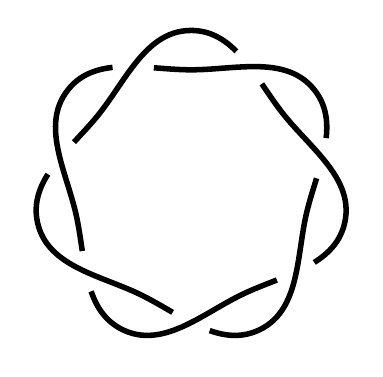
\begin{tikzpicture}[use Hobby shortcut]
        \path[spath/save=7-1]
        ([closed]90:2) foreach \k in {1,...,7} {
            .. (90-360/7+\k*720/7:1.5) .. (90+\k*720/7:2)
        } (90:2);
        \tikzset{
            every spath component/.style={draw},
            spath/knot={7-1}{15pt}{1,3,...,15}
        }
    \end{tikzpicture}
}

% --------------------------------------------------------------------
% Usage: \\SSTSincfoil
% --------------------------------------------------------------------
\newcommand{\SSTSincfoil}{%
    \begin{tikzpicture}
        \begin{knot}[
            consider self intersections=true,
    %        draft mode=crossings,
            flip crossing/.list={2,4},
            only when rendering/.style={
                show curve controls
            }
        ]
        \strand (2,0) .. controls +(0,1.0) and +(54:1.0) .. (144:2) .. controls +(54:-1.0) and +(18:-1.0) .. (-72:2) .. controls +(18:1.0) and +(162:-1.0) .. (72:2) .. controls +(162:1.0) and +(126:1.0) .. (-144:2) .. controls +(126:-1.0) and +(0,-1.0) .. (2,0);
        \end{knot}
    \end{tikzpicture}
}
% --------------------------------------------------------------------
% FigureEightDark: two circles, centers at (±D, 0), each radius = R (in cm)
% Usage: \SSTFigureEightDark
% Example: \SSTFigureEightDark
% --------------------------------------------------------------------
\newcommand{\SSTFigureEightDark}{%
    \begin{tikzpicture}[use Hobby shortcut]
        % ===== Up Quark knot (5_2): control points =====
        \coordinate (P1) at (-2.0,  -2.0);  % start / close
        \coordinate (P2) at (-2.0,  2.0);
        \coordinate (P3) at ( 1, -0.5);
        \coordinate (P4) at (-1, -0.5);
        \coordinate (P5) at ( 2.0,  2.0);
        \coordinate (P6) at ( 2.0, -2.0);
        \coordinate (P7) at (-1,  0.5);
        \coordinate (P8) at ( 1,  0.5);
        \coordinate (P9) at (-2.0, -2.0);  % = P1 (smooth closed path)

        \begin{knot}[
            consider self intersections,
            % draft mode=crossings,              % show crossing indices while tuning
            ignore endpoint intersections=false,
            clip width=5pt, clip radius=3pt,
            flip crossing/.list={2,4}        % same over/under pattern as your snippet
        ]
        \strand
        ([closed] P1)..(P2)..(P3)..(P4)..(P5)..(P6)..(P7)..(P8)..(P9);
        \end{knot}

    \end{tikzpicture}
}



% --------------------------------------------------------------------
% Hopf link: two circles, centers at (±D, 0), each radius = R (in cm)
% Usage: \SSTHopfLink[<flip list>]{<R cm>}{<D cm>}
% Example: \SSTHopfLink[2]{2}{1}
% --------------------------------------------------------------------
\newcommand{\SSTHopfLink}[3][2]{%
    \def\R{#2}\def\D{#3}%
    \begin{tikzpicture}
        \begin{knot}[
            consider self intersections,
            clip width=5pt, clip radius=3pt,
            ignore endpoint intersections=false,
            flip crossing/.list={#1}
        % draft mode=crossings
        ]
        \strand[sst/ring A] (\D,0)   circle[radius=\R cm];
        \strand[sst/ring B] (-\D,0)  circle[radius=\R cm];
        \end{knot}%
    \end{tikzpicture}%
}

% --------------------------------------------------------------------
% Borromean rings: three circles at vertices of an equilateral triangle
% Horizontal half-spacing = D (cm), so centers at:
%   ( +D, 0 ), ( -D, 0 ), ( 0, sqrt(3)*D )
% All radii = R (cm)
% Usage: \SSTBorromean[<flip list>]{<R cm>}{<D cm>}
% Example: \SSTBorromean[3,4]{2}{1}
% --------------------------------------------------------------------
\newcommand{\SSTBorromean}[3][3,4]{%
    \def\R{#2}\def\D{#3}%
    \begin{tikzpicture}
        \pgfmathsetmacro{\H}{\D*1.7320508075688772} % sqrt(3)*D
        \begin{knot}[
            consider self intersections,
            clip width=5pt, clip radius=3pt,
            ignore endpoint intersections=false,
            flip crossing/.list={#1}
        % draft mode=crossings
        ]
        \strand[sst/ring A] ( \D, 0)  circle[radius=\R cm];
        \strand[sst/ring B] (-\D, 0)  circle[radius=\R cm];
        \strand[sst/ring C] ( 0, \H)  circle[radius=\R cm];
        \end{knot}%
    \end{tikzpicture}%
}

% =========================
% Figure-8 knot (4_1)
% Usage: \SSTFigureEight[<flip list>]
% Default flip list matches your snippet: {1,3,5,7}
% =========================
\newcommand{\SSTFigureEight}[1][1,3,5,7]{%
    \begin{tikzpicture}[use Hobby shortcut]
        \begin{knot}[
            consider self intersections,
            clip width=6pt,
            clip radius=3pt,
            ignore endpoint intersections=false,
            flip crossing/.list={#1}
        % draft mode=crossings, % uncomment while tuning
        ]
        \strand
        ([closed]0,0)
        .. ( 1.5,  1.0)
        .. ( 0.5,  2.0)
        .. (-0.5,  1.0)
        .. ( 0.5,  0.0)
        .. ( 0.0, -0.5)
        .. (-0.5,  0.0)
        .. ( 0.5,  1.0)
        .. (-0.5,  2.0)
        .. (-1.5,  1.0)
        .. ( 0.0,  0.0);
        \end{knot}
        % small spacer to avoid clipping, matches your snippet
        \path (0,-.7);
    \end{tikzpicture}%
}

% =========================
% Trefoil (3_1), alternating 3 sides red / 3 sides blue
% This reproduces your "3 sides blue, 3 side red" using Hobby blanks + reuse.
% Usage: \SSTTrefoilAltColors
% (Scale from the surrounding tikzpicture if needed.)
% =========================
\newcommand{\SSTTrefoilAltColors}{%
    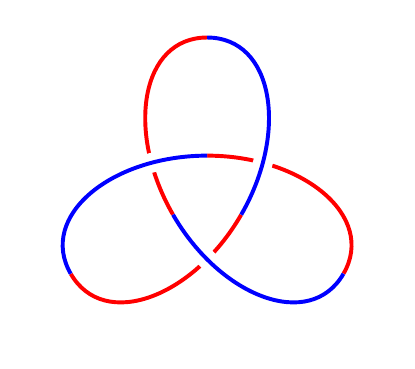
\begin{tikzpicture}[
        use Hobby shortcut,
        every path/.style={
            line width=1mm,
            white,
            double=red,
            double distance=.5mm
        }
    ]
        \def\nfoil{3}
        % base Hobby path with "soft" blanks at alternating arcs
        \draw ([closed]0,2)
        \foreach \k in {1,...,\nfoil} {
            .. ([blank=soft]90+360*\k/\nfoil-180/\nfoil:-.5)
            .. (90+360*\k/\nfoil:2)
        };
        % reuse the previous path with inverted blanks, drawn in blue
        \draw[
            use previous Hobby path={invert soft blanks,disjoint},
            double=blue
        ];
    \end{tikzpicture}%
}

% =========================
% Trefoil (3_1) via spath3 "knot" post-processor (two-color components)
% This reproduces your "1 side blue, 1 side red" approach.
% Usage: \SSTTrefoilSpath[<gap>][<flip list>]
% Defaults: gap=8pt, flips={1,3,5}
% =========================
\newcommand{\SSTTrefoilSpath}[2][8pt]{%
    \begin{tikzpicture}
        \begingroup
        \def\Gap{#1}%
        \def\Flips{#2}%
        % Saved spath named 'trefoil' (local to this group)
        \path[spath/save=trefoil]
        ([closed]90:2)
        \foreach \k in {1,...,3} {
            .. (-30+\k*240:.5) .. (90+\k*240:2)
        } (90:2);
        % Now render it as a knot with the requested gap + crossing flips
        \tikzset{spath/knot={trefoil}{\Gap}{\Flips}}
        \endgroup
    \end{tikzpicture}%
}
